%%%%%%%%%%%%%%%%%%%%%%%%%%%%%%%%%%%%%%%%%
% Beamer Presentation
% LaTeX Template
% Version 1.0 (10/11/12)
%
% This template has been downloaded from:
% http://www.LaTeXTemplates.com
%
% License:
% CC BY-NC-SA 3.0 (http://creativecommons.org/licenses/by-nc-sa/3.0/)
%
%%%%%%%%%%%%%%%%%%%%%%%%%%%%%%%%%%%%%%%%%

%----------------------------------------------------------------------------------------
%	PACKAGES AND THEMES
%----------------------------------------------------------------------------------------

\documentclass{beamer}
\usepackage{xcolor}
\usepackage{graphicx}
\usepackage{listings}
\usepackage{multicol}

\definecolor{applegreen}{rgb}{0.55, 0.71, 0.0}
\definecolor{blue(ncs)}{rgb}{0.0, 0.45, 0.60}
\definecolor{burgundy}{rgb}{0.5, 0.0, 0.13}


\mode<presentation> {

\usetheme{CambridgeUS}

\usecolortheme{wolverine}

\definecolor{gold}{HTML}{D4A017}
\definecolor{darkgold}{HTML}{B7950B}

\setbeamercolor{palette primary}{bg=gold,fg=white}
\setbeamercolor{palette secondary}{bg=darkgold,fg=white}
\setbeamercolor{palette tertiary}{bg=black,fg=white}
\setbeamercolor{palette quaternary}{bg=gold,fg=white}

\setbeamercolor{frametitle}{bg=darkgold,fg=white}

\setbeamercolor{section number projected}{bg=black,fg=gold}
\setbeamercolor{item}{fg=black,bg=gold}

\setbeamertemplate{page number in head/foot}[framenumber]
}

\usepackage{graphicx} % Allows including images
\usepackage{booktabs} % Allows the use of \toprule, \midrule and \bottomrule in tables

%----------------------------------------------------------------------------------------
%	TITLE PAGE
%----------------------------------------------------------------------------------------

\title[libCEED Finite Element Library]{Optimizing Performance for Portable Generic Finite Element Interfaces} % The short title appears at the bottom of every slide, the full title is only on the title page

\author{Jeremy L Thompson} % Your name
\institute[CU Boulder] % Your institution as it will appear on the bottom of every slide, may be shorthand to save space
{University of Colorado Boulder \\ % Your institution for the title page
\medskip
\textit{jeremy.thompson@colorado.edu} % Your email address
}
\date{\today} % Date, can be changed to a custom date

\begin{document}

%------------------------------------------------

\begin{frame}
\begin{center}
\frametitle{Machine Specs}

\begin{itemize}

\item CU Summit\\

~\\

\item Intel Xeon E5-2680 v3, 24 cores/node\\

~\\

\item Omni-Path HF1 interconnect\\

~\\

\item Using 4 full nodes (96 cores), no special location

\end{itemize}

\end{center}
\end{frame}

%------------------------------------------------

\begin{frame}
\begin{center}
\frametitle{BP 1 Pure C Backends}

\begin{multicols}{2}

\begin{flushleft}
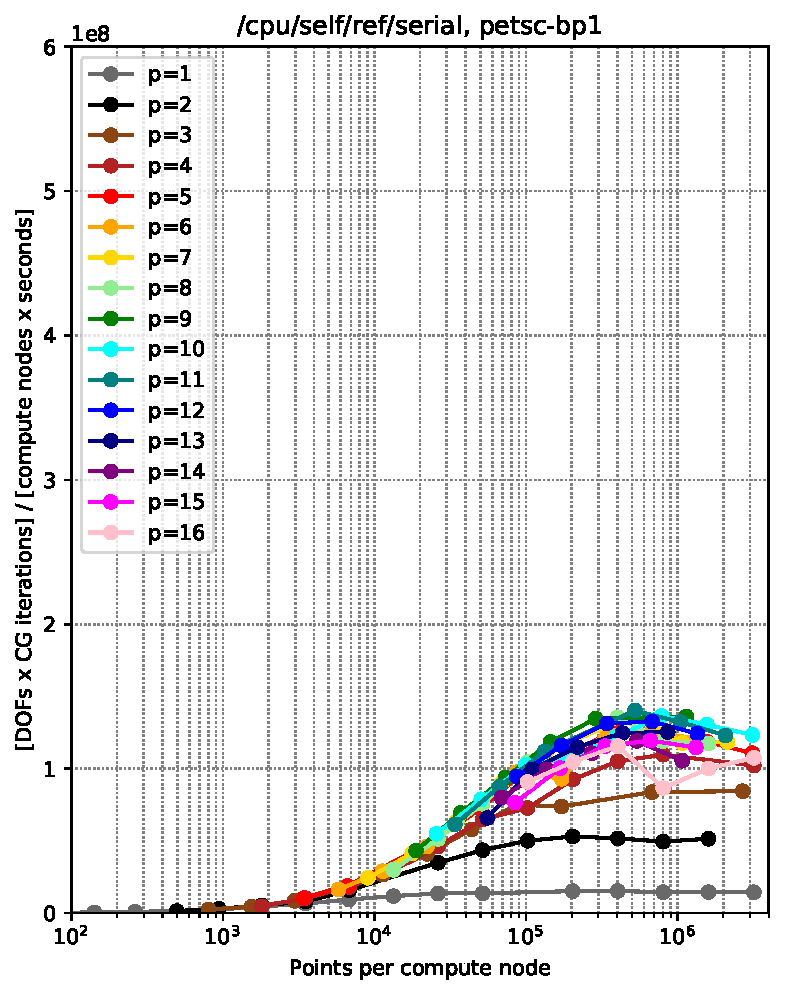
\includegraphics[width=5cm]{plot_libCEED_petsc-bp1_cpuselfrefserial_N004_pn24.pdf}
\end{flushleft}

\begin{flushright}
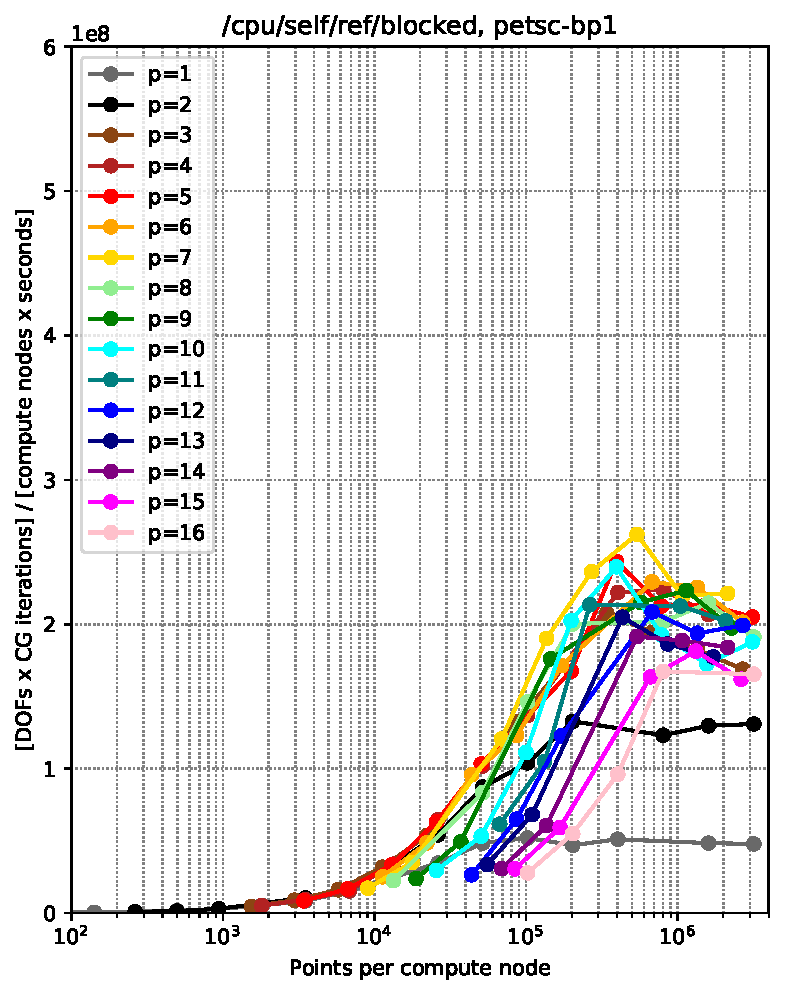
\includegraphics[width=5cm]{plot_libCEED_petsc-bp1_cpuselfrefblocked_N004_pn24.pdf}
\end{flushright}

\end{multicols}

\end{center}
\end{frame}

%------------------------------------------------

\begin{frame}
\begin{center}
\frametitle{BP 1 AVX Backends}

\begin{multicols}{2}

\begin{flushleft}
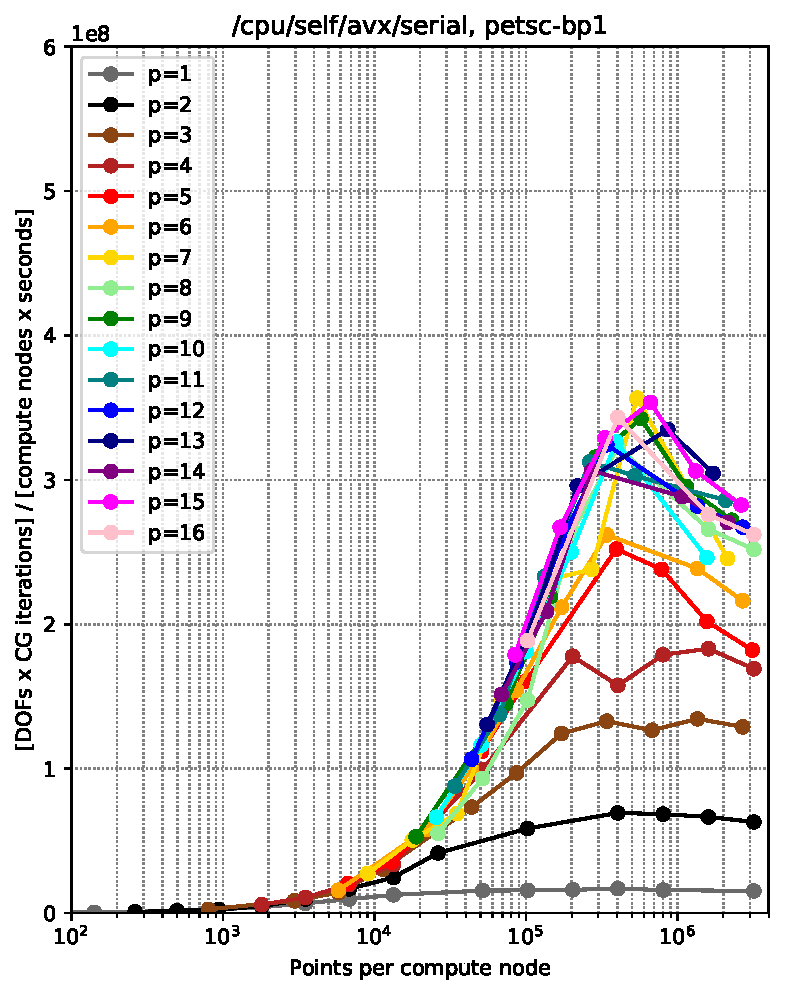
\includegraphics[width=5cm]{plot_libCEED_petsc-bp1_cpuselfavxserial_N004_pn24.pdf}
\end{flushleft}

\begin{flushright}
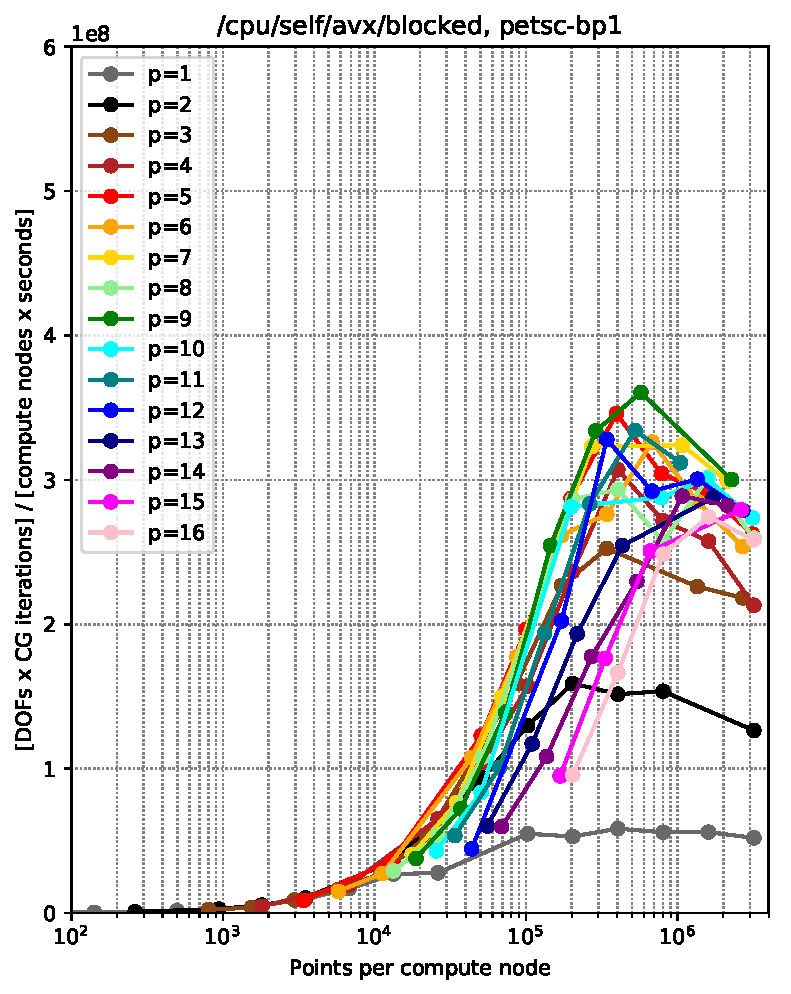
\includegraphics[width=5cm]{plot_libCEED_petsc-bp1_cpuselfavxblocked_N004_pn24.pdf}
\end{flushright}

\end{multicols}

\end{center}
\end{frame}

%------------------------------------------------

\begin{frame}
\begin{center}
\frametitle{BP 1 LIBXSMM Backends}

\begin{multicols}{2}

\begin{flushleft}
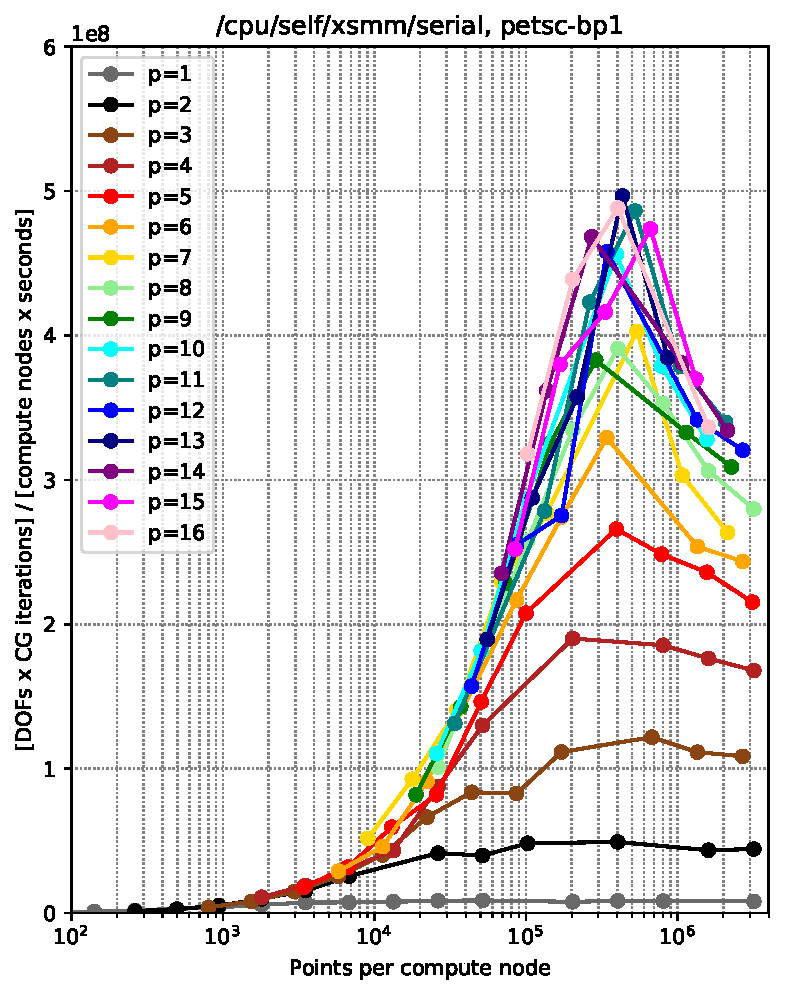
\includegraphics[width=5cm]{plot_libCEED_petsc-bp1_cpuselfxsmmserial_N004_pn24.pdf}
\end{flushleft}

\begin{flushright}
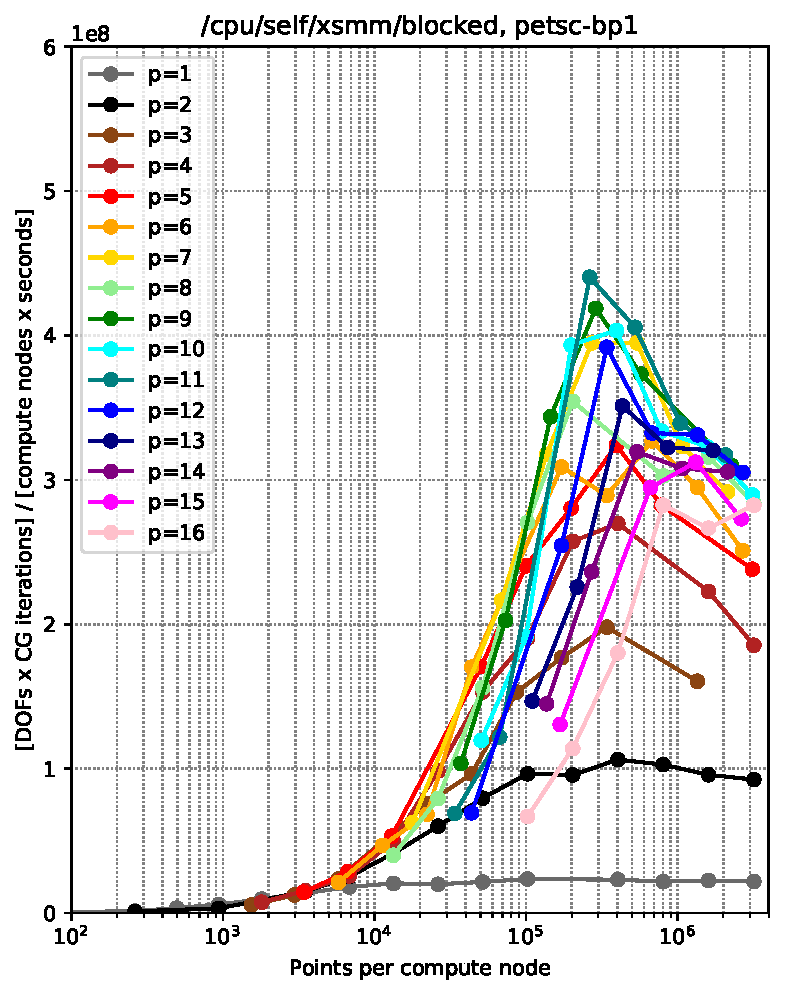
\includegraphics[width=5cm]{plot_libCEED_petsc-bp1_cpuselfxsmmblocked_N004_pn24.pdf}
\end{flushright}

\end{multicols}

\end{center}
\end{frame}

%------------------------------------------------

\begin{frame}
\begin{center}
\frametitle{BP 3 Pure C Backends}

\begin{multicols}{2}

\begin{flushleft}
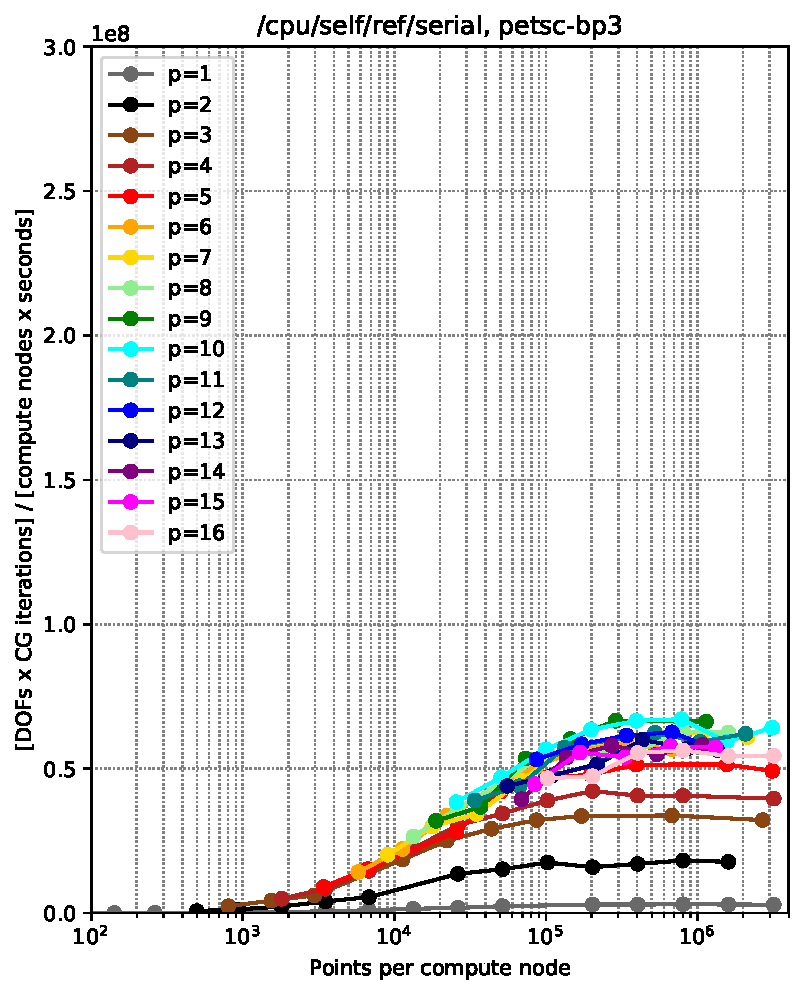
\includegraphics[width=5cm]{plot_libCEED_petsc-bp3_cpuselfrefserial_N004_pn24.pdf}
\end{flushleft}

\begin{flushright}
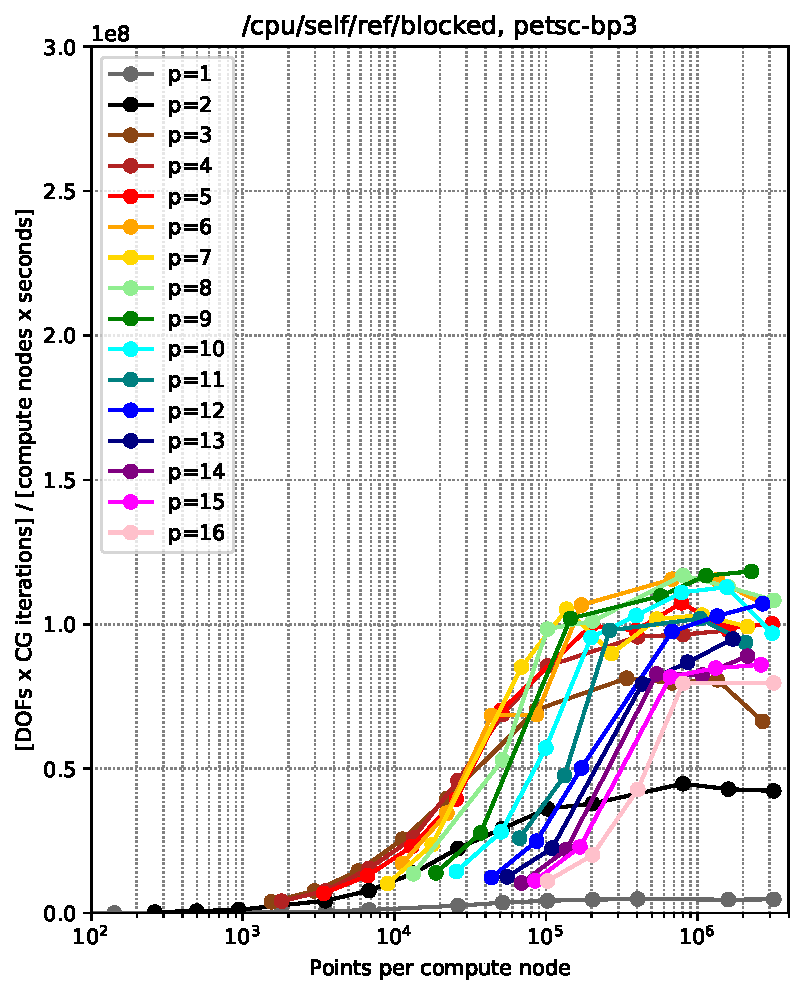
\includegraphics[width=5cm]{plot_libCEED_petsc-bp3_cpuselfrefblocked_N004_pn24.pdf}
\end{flushright}

\end{multicols}

\end{center}
\end{frame}

%------------------------------------------------

\begin{frame}
\begin{center}
\frametitle{BP 3 AVX Backends}

\begin{multicols}{2}

\begin{flushleft}
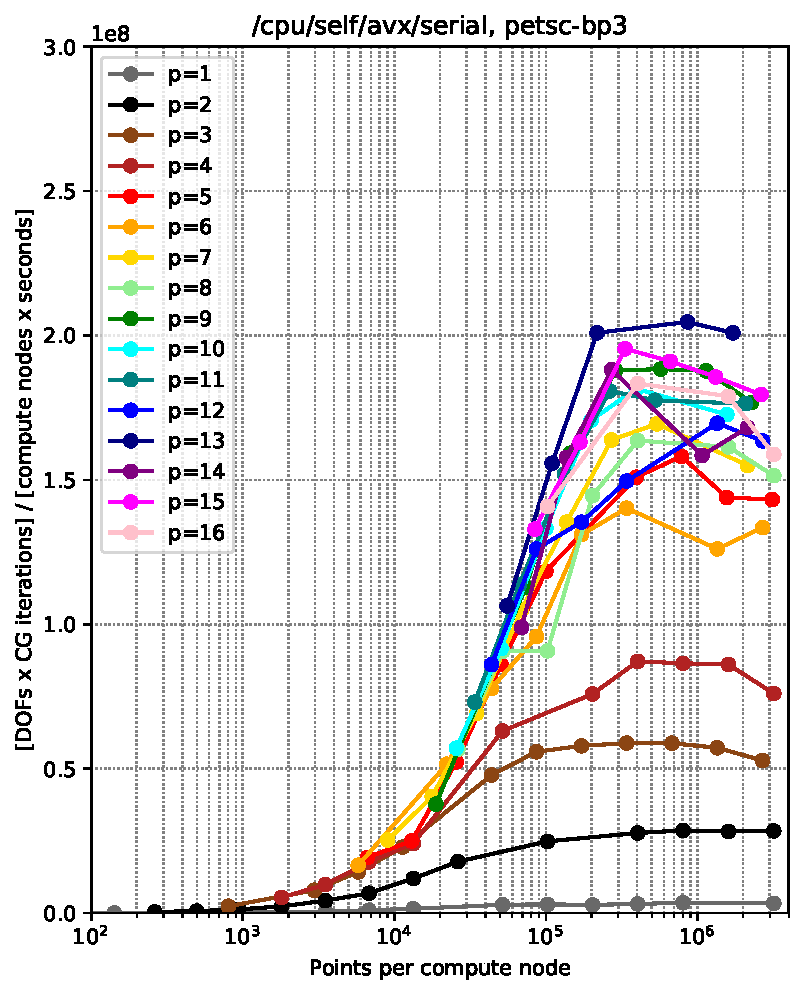
\includegraphics[width=5cm]{plot_libCEED_petsc-bp3_cpuselfavxserial_N004_pn24.pdf}
\end{flushleft}

\begin{flushright}
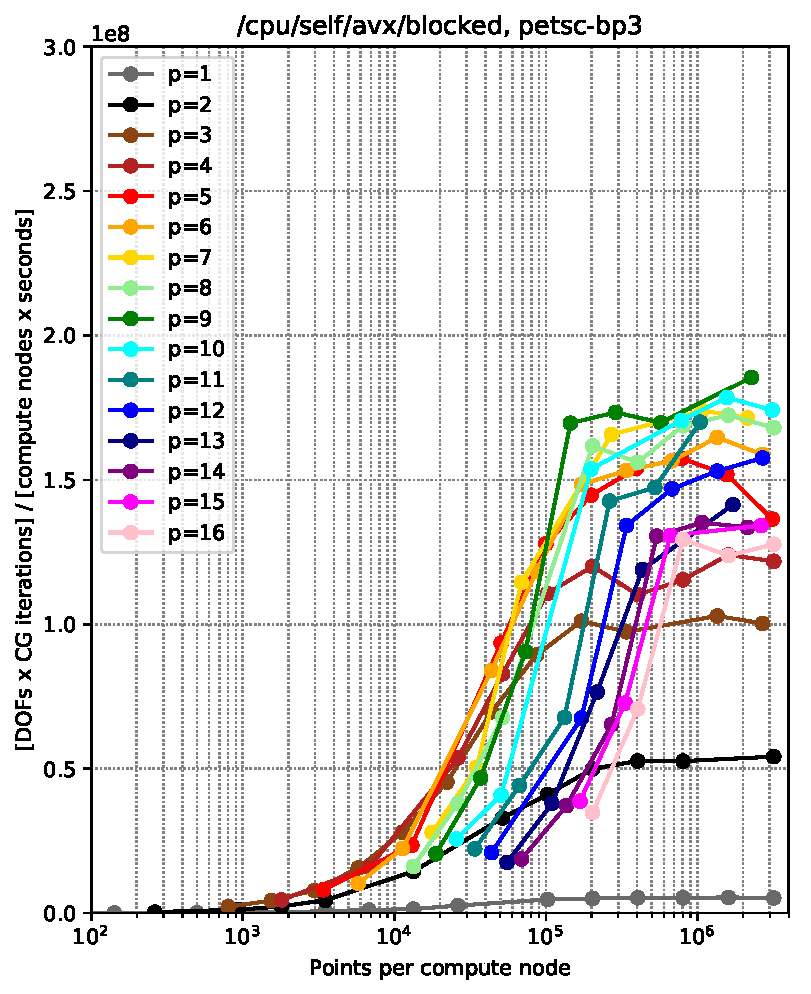
\includegraphics[width=5cm]{plot_libCEED_petsc-bp3_cpuselfavxblocked_N004_pn24.pdf}
\end{flushright}

\end{multicols}

\end{center}
\end{frame}

%------------------------------------------------

\begin{frame}
\begin{center}
\frametitle{BP 3 LIBXSMM Backends}

\begin{multicols}{2}

\begin{flushleft}
\includegraphics[width=5cm]{plot_libCEED_petsc-bp3_cpuselfxsmmserial_N004_pn24.pdf}
\end{flushleft}

\begin{flushright}
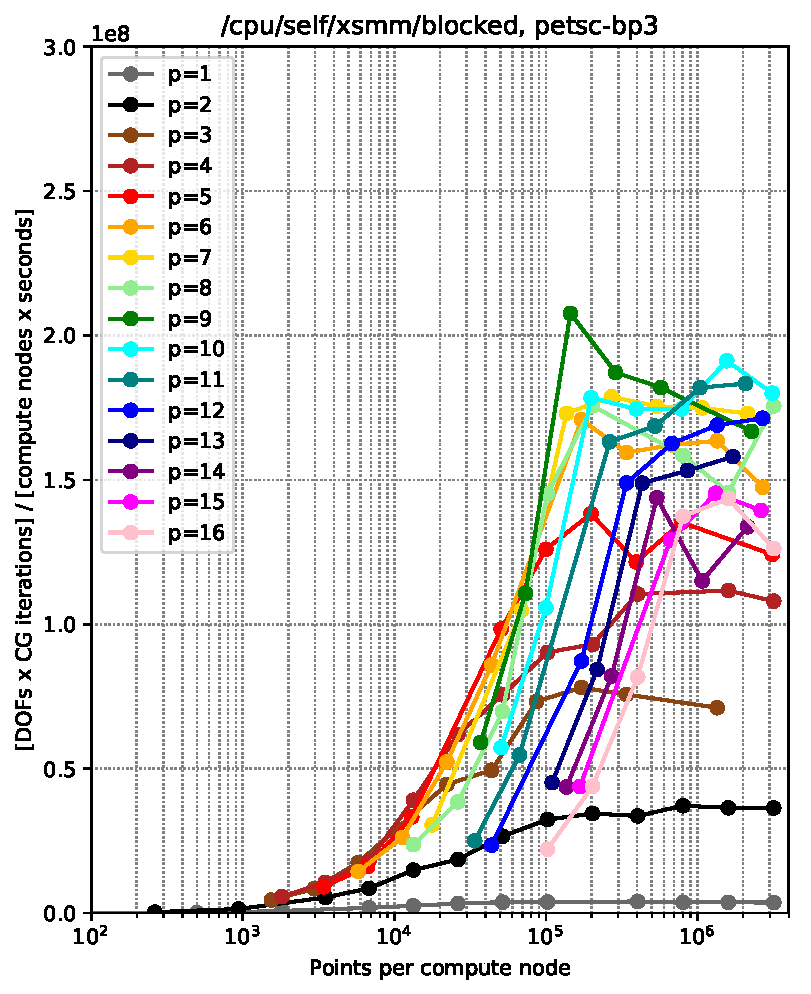
\includegraphics[width=5cm]{plot_libCEED_petsc-bp3_cpuselfxsmmblocked_N004_pn24.pdf}
\end{flushright}

\end{multicols}

\end{center}
\end{frame}

%------------------------------------------------

%----------------------------------------------------------------------------------------

\end{document}

